\documentclass[../main.tex]{subfiles}
\begin{document}

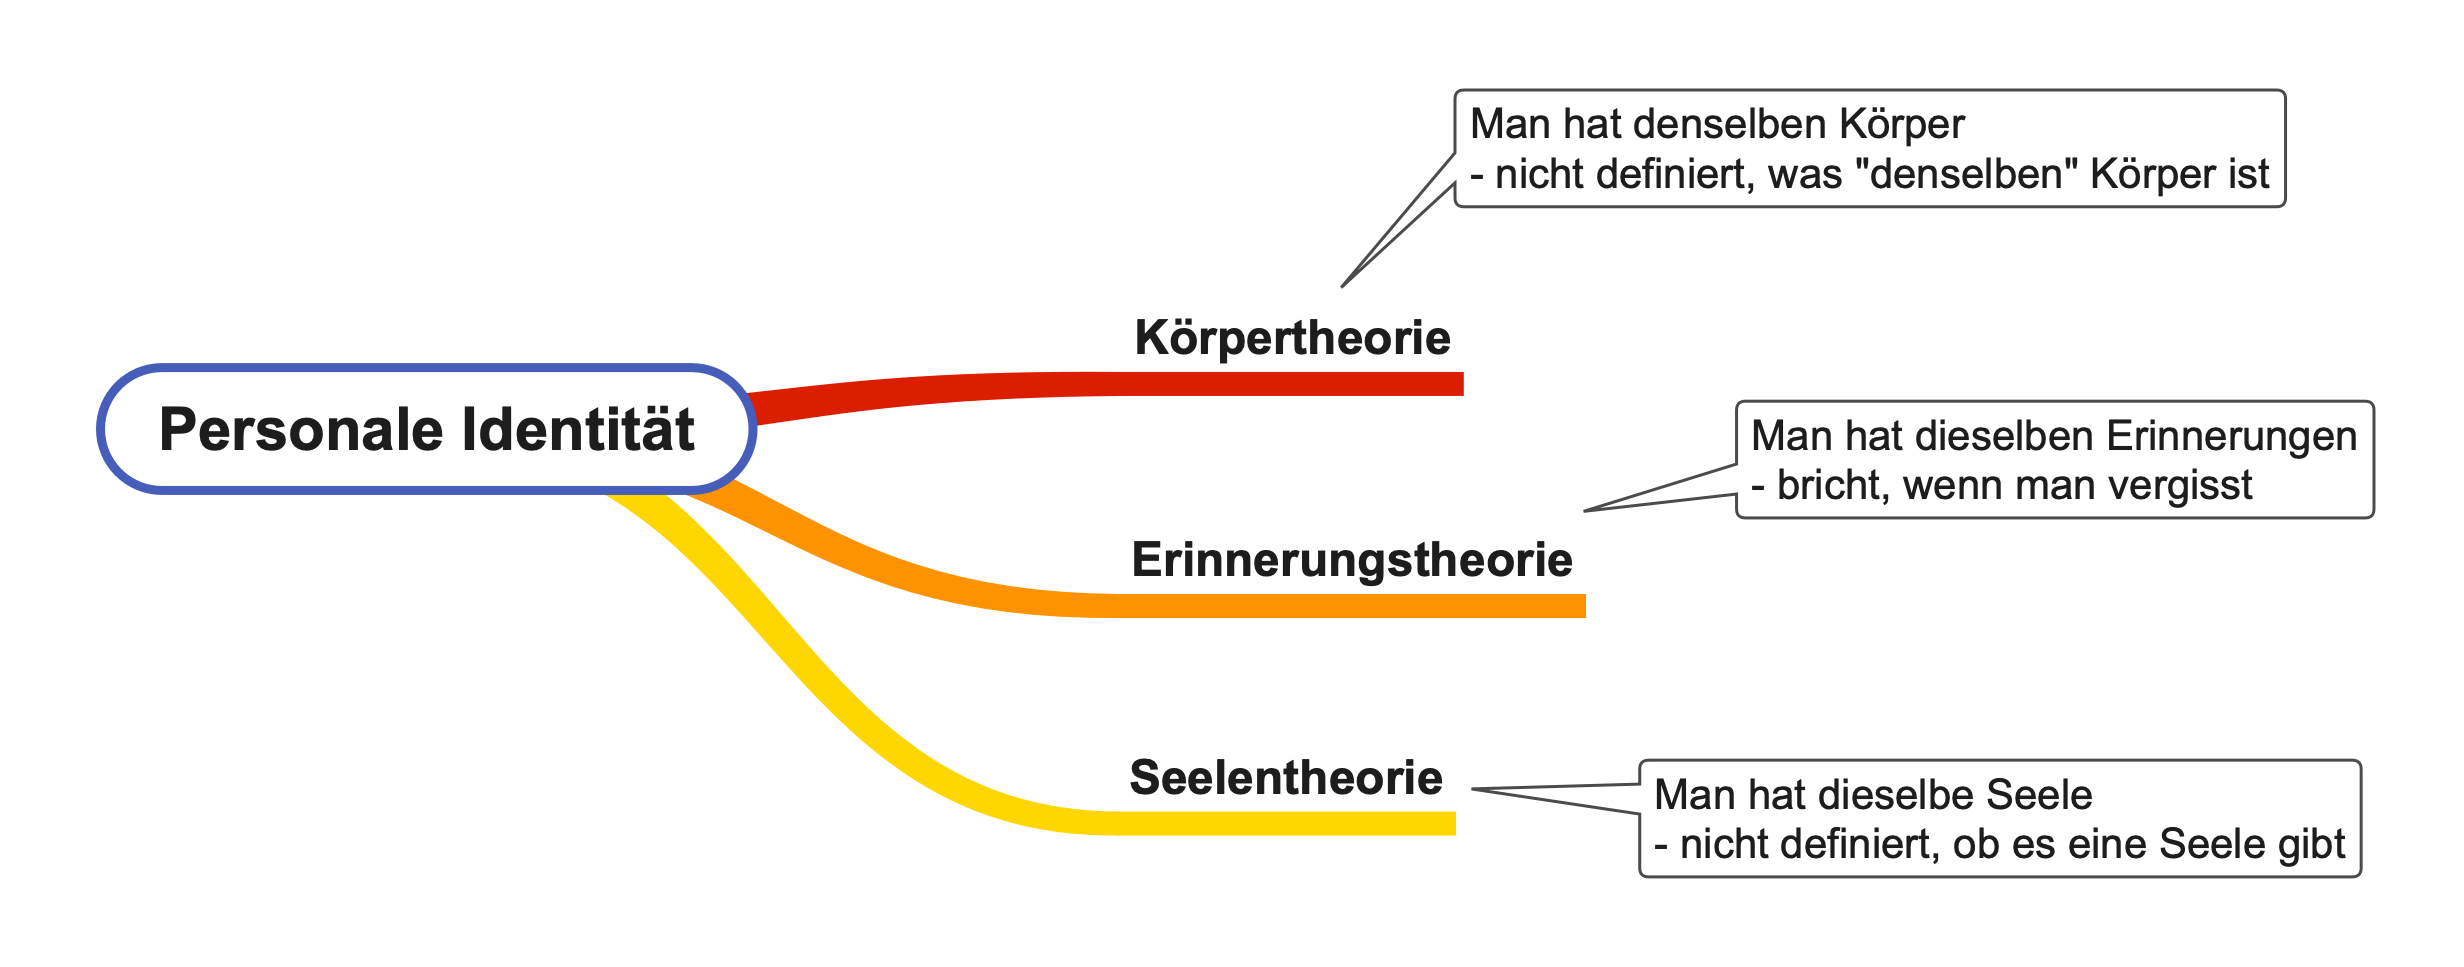
\includegraphics[width=\textwidth]{images/Personale_Identitaet_Uebersicht.png}

\paragraph{Problem} Sind wir die gleiche Person, wie vor fünf Minuten? Was genau macht es aus, dass ich ich bin? Oder in anderen Worten:\textit{Wenn ich aufgelöst/zerstört und an einem anderen Ort exakt gleich wieder zusammengesetzt werde, bin ich dann noch die gleiche Person?} oder \textit{Wenn ich ein Bild anschaue von mir selber vor 10 Jahren, sind wir noch die gleiche Person?}

\paragraph{Frage} Was ist dafür verantwortlich, dass ich ein und dieselbe Person bin?

\paragraph{Warum ist dies wichtig?} Besonders das Strafrecht interessiert sich dafür; \textit{A hat sich straffällig gemacht, ist nun B die gleiche Person, die ich bestrafen würde?}

\section{Was ist personale Identität?}\label{SectionPersonaleIdentitaet}
Personale Identität ist numerische Identität (siehe \ref{gD:numUndqualIdent}) über Zeit, also \textbf{diachrone numerische Identität}. Eine qualitative Identität kann sie nicht sein, denn mein momentanes Ich und das Ich vor einer Zeitspanne müssen nicht die gleichen Eigenschaften haben.

\subsection{Körpertheorie der personalen Identität}
\paragraph{These} A ist dieselbe Person wie B, gdw. beide den gleichen Körper haben. 
\paragraph{Problem} 
\begin{enumerate}
	\item Es ist unklar, was die notwendigen und hinreichenden Bedingungen dafür sind, dass A und B denselben Körper haben. 
\end{enumerate}

\subsection{Erinnerungstheorie der personalen Identität}
\paragraph{These} A ist dieselbe Person wie B, gdw. B (oder A) sich an dieselben Erlebnisse/mentalen Zustände wie A (oder B) erinnern kann. 
\paragraph{Problem} 
\begin{enumerate}
	\item Die Definition scheint unvollständig, da B (oder A) sich nicht zwingend an alles erinnern kann/muss wie A (oder B). So zum Beispiel im Falle einer Krankheit oder durch schlichtes Vergessen, resp. gar nicht erst Aufnehmen.
\end{enumerate}

\subsection{Seelentheorie der personalen Identität}
\paragraph{These} A ist dieselbe Person wie B, gdw. die immaterielle Seele von A dieselbe ist wie die immaterielle Seele von B.
\paragraph{Problem} 
\begin{enumerate}
	\item Das Vorhandensein einer immaterielle Seele wird in Frage gestellt. 
\end{enumerate}


\end{document}